\section{Efficient text-search using TF-IDF}

TF-IDF stands for Term Frequency-Inverse Document Frequency. 
The TF-IDF weight is a weight often used in information 
retrieval and text mining. Variations of the TF-IDF weighting 
the scheme is often used by search engines in scoring and ranking 
a document’s relevance given a query. 
This weight is a statistical measure used to evaluate how 
important a word is to a document in a collection or corpus. 
The importance increases proportionally to the number of times 
a word appears in the document but is offset by the frequency 
of the word in the corpus.

TF-IDF is a weighting scheme that assigns each term in a 
document a weight based on its Term Frequency (TF) and 
Inverse Document Frequency (IDF). The terms with higher weight scores are considered to be more important.

Typically, the TF-IDF weight is composed by two terms:
\begin{enumerate}
    \item Normalized Term Frequency (TF)
    \item Inverse Document Frequency (IDF)
\end{enumerate}

Therefore, Term Frequency is a measure of how frequently a 
term occurs in a document.
\begin{equation}
    tf(t, D) = \frac{\text{Number of times the term } t \text{ appears in document } D}{\text{Total number of terms in the document}}
    \label{eqn:tf}
\end{equation}

Inverse Document Frequency is a measure of how important a term is.~\cite{tfidftutorial}
\begin{equation}
    idf(t, D) = \log \frac{N}{n _t}
    \label{eqn:idf}
\end{equation}
where, $N =$ Total number of documents, $n _t =$ Number of documents having the term $t$ in it.

Now combine both to produce a composite weight for each term in each document.
\begin{equation}
    tfidf(t,D) = tf(t,D) \times idf(t,D)
    \label{eqn:tfidf}
\end{equation}
Also, The TF-IDF score/relevancy for a multi-term query $q = (t 1 , . . . , t_m)$ is~\cite{tfidfFormulae}:
\begin{equation}
    score _{tfidf}(q, d, D) = \sum^{m}_{i = 1} score _{tfidf}(t _i, d, D)
    \label{eqn:score}
\end{equation}

\subsubsection{Use of TF-IDF text search in an example}

Suppose a search engine contained the following three documents,

\textbf{Document A:} "the mouse played with the cat"

\textbf{Document B:} "the quick brown fox jumped over the lazy dog"

\textbf{Document C:} "dog 1 and dog 2 ate the hot dog"

The TF-IDF vector is now computed for each document like so~\cite{tfidfExample}:

\textbf{Document A:} "the mouse played with the cat"
\begin{figure}[h!]
    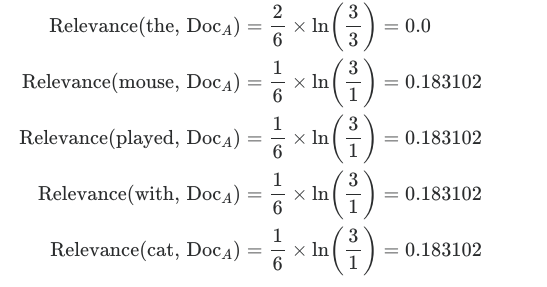
\includegraphics[width=10cm]{tfidf-example.png}
\end{figure}

\subsection{Compare query against document}
\begin{enumerate}
    \item Find the TF-IDF vector for the document. This should be an easy, $O(1)$ lookup since the TF-IDF vector was already computed.
    \item Compute the TF-IDF vector for the query. (Note: technically, the query is treated as if it were a new document. 
    However, the IDF values need not be recomputed: just use the ones computed earlier.)
    \item Compute the cosine similarity between the document vector and the query vector.
    \item This can be done by comparing the TF-IDF vector for the query against all the document TF-IDF vectors and compute how similar the query vector is to each document by exploiting properties of the cosine function and the dot product.
\end{enumerate}

The $K$ documents of the collection with the highest vector space scores on the query $q$ need to be determined. Typically, these $K$ top documents ordered by the score in decreasing order is what is needed; for instance, many search engines use $K = 10$ to retrieve and rank-order the first page of the ten best results.~\cite{tfidfExample}

\subsubsection{Time Complexity}

The time complexity of this algorithm is:
\begin{equation}
    O(|Q| |D| |T|) = O(|D| |T|)
\end{equation}

where $|Q|$ is considered fixed, $Q$ is the set of words in the query and $D$ is the set of all documents.

Also, if the $D$ is the set of only the matching documents, then
since scores is a priority queue (at least in doc-at-time-scheme) built on the heap, 
putting every $d$ into takes $\log K$. Therefore, an estimate can be $O(|D| \log K )$.~\cite{tfidfComplexity}

